%\documentclass[usenames,dvipsnames,12pt,handout]{beamer}
\documentclass[usenames,dvipsnames,12pt]{beamer}

\usecolortheme{dove}
\usefonttheme{professionalfonts}
\usefonttheme{serif}

\usepackage{bm}
\usepackage{mathtools}
\usepackage{amsmath,amssymb,amsfonts,amsthm}
\usepackage{mathrsfs}
\usepackage{mathabx}
\usepackage{fontspec}
\usepackage{multicol}
\usepackage{xcolor}
\usepackage{pifont}
\usepackage{tabularx}
\usepackage{colortbl}
\usepackage{graphicx}
\usepackage{semantic}
\usepackage{xspace}
\usepackage[all]{xy}
\usepackage{listings}
\usepackage{lstautogobble}
\usepackage{fancybox}
\usepackage{stmaryrd}
\usepackage{rotating}
\usepackage{wasysym}
\usepackage{ulem}
\usepackage{soul}
\usepackage{newunicodechar}
\usepackage[super]{nth}
\usepackage{tikz, tikz-qtree, tikz-qtree-compat}
\usetikzlibrary{shapes, arrows, calc, quotes, tikzmark, decorations.pathreplacing, decorations.markings}
\usepackage{makecell}
\usepackage{epigraph}

\setlength{\multicolsep}{3pt}
\setlength{\columnseprule}{0.5pt}

\newcommand\mytikzmark[2]{\tikz[overlay,remember picture, anchor=base] \node (#1) {#2};}

% colored underline, with Beamer overlay support
% usage: \cul{x} or \cul[blue]{x} or \cul<2->{x} or \cul<2->[blue]{x}
\newcommand<>{\cul}[2][Red]{
  \fontdimen8\textfont3=0.75pt
  \alt#3
      {\color{#1}\underline{{\color{black}#2}}\color{black}}
      {\transparent{0.0}\underline{{\transparent{1.0}#2}}\transparent{1.0}}
}
\newcommand{\smalltt}[1]{{\small \texttt{#1}}}
\newcommand{\McL}{\mathscr{L}}
\newcommand{\yes}{\textcolor{Green}{\ding{51}}}
\newcommand{\no}{\textcolor{Red}{\ding{55}}}
\newcommand{\maybe}{\ding{82}}
\newcommand{\redtext}[1]{\textcolor{Maroon}{#1}}
\newcommand{\bluetext}[1]{\textcolor{NavyBlue}{#1}}
\newcommand{\orangetext}[1]{\textcolor{BurntOrange}{#1}}
\newcommand{\greentext}[1]{\textcolor{PineGreen}{#1}}
\newcommand{\graytext}[1]{\textcolor{gray}{#1}}
\newcommand{\purpletext}[1]{\textcolor{Plum}{#1}}
\newcommand{\bl}[1]{\ensuremath{\orangetext{#1}}}
\newcommand{\key}[1]{\ensuremath{\mathtt{#1}}}
\newcommand{\MID}{\;\mid\;}
\newcommand{\Surface}{\ensuremath{\lambda_{\mathtt{IFC}}^\star}\xspace}
\newcommand{\SurfaceOld}{\ensuremath{\lambda_{\mathtt{SEC}}^\star}\xspace}
\newcommand{\CCOld}{\ensuremath{\lambda_{\mathtt{SEC}}^{\Rightarrow}}\xspace}
\newcommand{\CC}{\ensuremath{\lambda_{\mathtt{IFC}}^{c}}\xspace}
\newcommand{\GSLRef}{\ensuremath{\mathrm{GSL}_\mathsf{Ref}}\xspace}
\newcommand{\GSLRefEps}{\ensuremath{\mathrm{GSL}_\mathsf{Ref}^\epsilon}\xspace}
\newcommand{\SSLRef}{\ensuremath{\mathrm{SSL}_\mathsf{Ref}}\xspace}
\newcommand{\lamgif}{\ensuremath{\mathit{\lambda_{gif}}}\xspace}
\newcommand{\WHILEG}{WHILE\textsuperscript{G}\xspace}
\newcommand{\high}{\textcolor{OrangeRed}{\key{high}}\xspace}
\newcommand{\low}{\textcolor{PineGreen}{\key{low}}\xspace}
\newcommand{\unk}{\textcolor{Maroon}{\key{\star}}\xspace}
\newcommand{\Bool}{\key{Bool}}
\newcommand{\Int}{\key{Int}}
\newcommand{\Unit}{\key{Unit}}
\newcommand{\Fun}[3]{\ensuremath{{#1}\xrightarrow{{#2}}{#3}}}
\newcommand{\Refer}[1]{\ensuremath{\key{Ref}\;{#1}}}
\newcommand{\true}{\key{true}}
\newcommand{\false}{\key{false}}
\newcommand{\unit}{\key{unit}}
\newcommand{\pc}{\ensuremath{\mathit{pc}}\xspace}
\newcommand{\PC}{\ensuremath{\mathit{PC}}\xspace}
\newcommand{\gc}{\ensuremath{\mathit{gc}}\xspace}
\newcommand{\syntax}[1]{\text{\texttt{\textcolor{Purple}{#1}}}}
\newcommand{\ccsyntax}[1]{\text{\texttt{{#1}}}}
\newcommand{\const}[2]{\ensuremath{\syntax{(\$}\;{#1}\syntax{)}_{#2}}}
\newcommand{\lam}[5]{\ensuremath{\syntax{(λ}^{#1}{#2}\syntax{:}{#3}\syntax{.}\,{#4}\syntax{)}_{#5}}}
\newcommand{\app}[3]{\ensuremath{\syntax{(}{#1}\;{#2}\syntax{)}^{\bl{#3}}}}
\newcommand{\ifexp}[4]{\ensuremath{\syntax{(if}\;{#1}\;\syntax{then}\;{#2}\;\syntax{else}\;{#3}\syntax{)}^{\bl{#4}}}}
\newcommand{\refexp}[3]{\ensuremath{\syntax{(ref}\;{#1}\;{#2}\syntax{)}^{\bl{#3}}}}
\newcommand{\deref}[1]{\ensuremath{\syntax{!}\;{#1}}}
\newcommand{\assign}[3]{\ensuremath{\syntax{(}{#1}\;\syntax{:=}\;{#2}\syntax{)}^{\bl{#3}}}}
\newcommand{\ann}[3]{\ensuremath{\syntax{(}{#1}\;\syntax{:}\;{#2}\syntax{)}^{\bl{#3}}}}
\newcommand{\letexp}[3]{\ensuremath{\syntax{let}\;{#1}={#2}\;\syntax{in}\;{#3}}}
\newcommand{\ccconst}[1]{\ensuremath{\ccsyntax{\$}\;{#1}}}
\newcommand{\ccaddr}[1]{\ensuremath{\ccsyntax{addr}\;{#1}}}
\newcommand{\cclam}[2]{\ensuremath{\ccsyntax{λ}{#1}\ccsyntax{.}\,{#2}}}
\newcommand{\ccif}[5]{\ensuremath{\ccsyntax{if}\;{#1}\;{#2}\;{#3}\;{#4}\;{#5}}}
\newcommand{\ccifstar}[4]{\ensuremath{\ccsyntax{if}{\star}\,{#1}\,{#2}\,{#3}\,{#4}}}
\newcommand{\ccref}[2]{\ensuremath{\ccsyntax{ref}\;{#1}\;{#2}}}
\newcommand{\ccrefproj}[3]{\ensuremath{\ccsyntax{ref?}^{\bl{#3}}\;{#1}\;{#2}}}
\newcommand{\ccderef}[3]{\ensuremath{\ccsyntax{!}\;{#1}\;{#2}\;{#3}}}
\newcommand{\ccderefstar}[2]{\ensuremath{\ccsyntax{!}{\star}\,{#1}\,{#2}}}
\newcommand{\ccassign}[5]{\ensuremath{\ccsyntax{assign}\;{#1}\;{#2}\;{#3}\;{#4}\;{#5}}}
\newcommand{\ccassignproj}[5]{\ensuremath{\ccsyntax{assign?}^{\bl{#5}}\;{#1}\;{#2}\;{#3}\;{#4}}}
\newcommand{\cccast}[2]{\ensuremath{{#1}\,\ccsyntax{⟨}\,{#2}\,\ccsyntax{⟩}}}
\newcommand{\ccprot}[4]{\ensuremath{\ccsyntax{prot}\;{#1}\;{#2}\;{#3}\;{#4}}}
\newcommand{\cccastpc}[2]{\ensuremath{\ccsyntax{cast}_{\ccsyntax{pc}}\;{#1}\;{#2}}}
\newcommand{\cclet}[4]{\ensuremath{\ccsyntax{let}\;{#1}\ccsyntax{=}{#2}\ccsyntax{:}{#3}\;\ccsyntax{in}\;{#4}}}
\newcommand{\ccapp}[5]{\ensuremath{\ccsyntax{app}\;{#1}\;{#2}\;{#3}\;{#4}\;{#5}}}
\newcommand{\ccappstar}[4]{\ensuremath{\ccsyntax{app}{\star}\,{#1}\,{#2}\,{#3}\,{#4}}}
\newcommand{\ccopaque}{\ensuremath{\ccsyntax{●}}}
\newcommand{\lconsisjoin}{\ensuremath{\,\widetilde{\curlyvee}\,}}  % label consistent join
\newcommand{\consisjoin}{\ensuremath{\,\widetilde{\vee}\,}}        % type consistent join
\newcommand{\lconsismeet}{\ensuremath{\,\widetilde{\curlywedge}\,}}  % label consistent meet
\newcommand{\consismeet}{\ensuremath{\,\widetilde{\wedge}\,}}        % type consistent meet
\newcommand{\Cast}[3]{\ensuremath{{#1}\Rightarrow^{\bl{#3}}{#2}}}
\newcommand{\Type}{\textit{Type}}
\newcommand{\RawType}{\textit{RawType}}
\newcommand{\Label}{\textit{Label}}
\newcommand{\compile}[1]{\ensuremath{\mathcal{C}\;{#1}}}
\newcommand{\applycast}[3]{\ensuremath{\mathbf{Cast}\;{#1}\,,\,{#2}\leadsto{#3}}}
\newcommand{\blame}[1]{\ensuremath{\key{blame}\;\bl{#1}}}
\newcommand{\reduce}[5]{\ensuremath{{#1}\mid{#2}\mid{#3}\longrightarrow{#4}\mid{#5}}}
\newcommand{\Active}[1]{\ensuremath{\mathbf{Active}\;{#1}}}
\newcommand{\Inert}[1]{\ensuremath{\mathbf{Inert}\;{#1}}}
\newcommand{\bigstep}[5]{\ensuremath{{#1}\mid{#2}\vdash{#3}\Downarrow{#4}\mid{#5}}}
\newcommand{\bigstepe}[5]{\ensuremath{{#1}\mid{#2}\vdash{#3}\Downarrow_\epsilon{#4}\mid{#5}}}
%% coercions
\newcommand{\id}[1]{\ensuremath{\mathit{\bold{id}}(#1)}}
\newcommand{\up}{\ensuremath{\boldsymbol{\uparrow}}}
\newcommand{\inj}[1]{\ensuremath{{#1}\,\boldsymbol{!}}}
\newcommand{\seq}{\ensuremath{\,\boldsymbol{;}\,}}
\newcommand{\err}[3]{\ensuremath{\boldsymbol{\bot}^{\bl{#3}}\;{#1}\;{#2}}}
\newcommand{\proj}[2]{\ensuremath{{#1}\,\boldsymbol{?}^{\bl{#2}}}}
\newcommand{\coerc}[2]{\ensuremath{{#1}\boldsymbol{,}\,{#2}}}
\newcommand{\refco}[2]{\ensuremath{\mathbf{Ref}\;{#1}\;{#2}}}
\newcommand{\funco}[3]{\ensuremath{{#1}\boldsymbol{,}\,{#2}\boldsymbol{\rightarrow}{#3}}}
\newcommand{\precctx}[8]{\ensuremath{{#1};{#2};{#3};{#4};{#5};{#6};{#7};{#8}}}
\newcommand{\ccprec}[4]{\ensuremath{\vdash{#1}\sqsubseteq{#2}\Leftarrow{#3}\sqsubseteq{#4}}}

\newcommand{\highlight}[2]{\colorbox{#1}{\ensuremath{#2}}}
\newcommand{\highlightblue}[1]{\highlight{White!90!NavyBlue}{#1}}
\newcommand{\highlightred}[1]{\highlight{White!90!Maroon}{#1}}

\definecolor{highlight}{gray}{0.9}

\newunicodechar{ℒ}{\ensuremath{\McL}}
\newunicodechar{𝕋}{\ensuremath{\mathbb{T}}}
\newunicodechar{𝕊}{\ensuremath{\mathbb{S}}}

\newtheorem{conjecture}[theorem]{\translate{Conjecture}}
%\newtheorem{theorem}{Theorem}
%\newtheorem{lemma}[theorem]{Lemma}
%\newtheorem{corollary}[theorem]{Corollary}
\newtheorem{proposition}[theorem]{Proposition}
\newtheorem{constraint}[theorem]{Constraint}
%\newtheorem{definition}[theorem]{Definition}
%\newtheorem{example}[theorem]{Example}

%% Configurations:
\setmainfont{EB Garamond}
\setmonofont[Scale=0.9]{Iosevka}
\setbeamertemplate{navigation symbols}{}
\setbeamertemplate{footline}[frame number]
\setbeamerfont{footnote}{size=\tiny}
\setlength{\multicolsep}{3pt}
\setbeamertemplate{itemize item}{$\blacktriangleright$}
\setbeamertemplate{itemize subitem}{$\circ$}
\setbeamertemplate{itemize/enumerate subbody begin}{\footnotesize}

\lstdefinestyle{mystyle}{
  commentstyle=\color{Green},
  keywordstyle=\color{Magenta},
  numberstyle=\tiny\color{Gray},
  stringstyle=\color{Purple},
  basicstyle=\ttfamily\small,
  breakatwhitespace=false,
  breaklines=true,
  captionpos=b,
  keepspaces=true,
  numbers=left,
  numbersep=5pt,
  showspaces=false,
  showstringspaces=false,
  showtabs=false,
  tabsize=2
}

\lstset{style=mystyle}

\setlength{\epigraphwidth}{\textwidth}


\title{The Holy Grail of Gradual Security \\
  {\small\textcolor{NavyBlue}{Ph.D Thesis Proposal Presentation}} \vspace{-15pt}}
\author{Tianyu Chen}
\institute{\small Computer Science, Indiana University}
\date{}

\begin{document}

%%%%%%%%%% Cover Page %%%%%%%%%%%
\begin{frame}
  \titlepage
  \begin{tikzpicture}[remember picture,overlay]
    \node [anchor=north east] at ([xshift=-15pt, yshift=5pt]current page.north east)
          {
\includegraphics[height=30pt]{iu_tab_web}};
  \end{tikzpicture}

  \vspace{-45pt}

  \begin{center}
    
\includegraphics[width=4in]{acanthus}
  \end{center}

  \footnotetext{Acanthus textiles. William Morris Gallery}
\end{frame}

%%%%%%%%%% Road Map %%%%%%%%%%%
\begin{frame}
  \frametitle{Road Map}

  \begin{itemize}
  \item[\textcolor{Red}{\ding{43}}] \cul{Background:}
    \begin{itemize}
    \item Explicit flow and implicit flow
    \item Information flow control (IFC), static and dynamic
    \item The tension between IFC and gradual typing
    \end{itemize}
  \item \Surface in Action
    \begin{itemize}
    \item[\ding{79}] Solving the Tension Between Noninterference and the Gradual Guarantee
    \item Type-Based Reasoning in \Surface
    \end{itemize}
  \item Coercion-based Semantics for Gradual Security
  \item Meta-theoretical Results of \Surface
  \end{itemize}
\end{frame}

%%%%%%%%%% Explicit Information Flow %%%%%%%%%%%
\begin{frame}[fragile]
  \frametitle{Explicit Information Flow}

  Can we infer output from input in the following program?

\begin{verbatim}
let input = private-input () in publish (¬ input)
\end{verbatim}

\onslide<2-> {
  \begin{itemize}
  \item[\yes] Yes!
  \item Witness at least two executions
  \item Output is the negation of input
  \item \purpletext{Explicit flow}
  \end{itemize}
}

\end{frame}

%%%%%%%%%% Implicit Information Flow %%%%%%%%%%%
\begin{frame}[fragile]
  \frametitle{Implicit Information Flow}

  Can we infer output from input in the following program?
\begin{verbatim}
  let input = private-input () in
      publish (if input then false else true)
\end{verbatim}

\onslide<2-> {
\begin{itemize}
  \item[\yes] Also yes
  \item Again, output is the negation of input
  \item \purpletext{Implicit flow}: input influences output through {\large\textit{branching}}
\end{itemize}
}

\end{frame}

%%%%%%%%%% IFC %%%%%%%%%%%
\begin{frame}
  \frametitle{Information-Flow Control (IFC)}

  \begin{itemize}
  \item Ensures that information transfers adhere to a security policy
    \item For example, \high input must not flow to \low output
    \item Propagate and check the security labels
    \item IFC in PL
      \(
      \left\{
      \begin{minipage}[c]{0.75\linewidth}
      \item[] \bluetext{\Huge static} using a type system
      \item[] \redtext{\Huge dynamic} using runtime monitoring
      \end{minipage}
      \right.
      \)
  \end{itemize}
\end{frame}

%%%%%%%%%% Static IFC, Explicit Flow %%%%%%%%%%%
\begin{frame}[containsverbatim]
  \frametitle{\bluetext{Static IFC} Accepts \textcolor{Green}{Legal} Explicit Flow}

  (Static IFC using a type system)
  \begin{lstlisting}[mathescape,autogobble,xleftmargin=.15\textwidth,xrightmargin=.15\textwidth]
    let fconst = λ b : $\Bool_{\high}$. false in
    let input  = private-input () in
    let result = fconst input in
      publish result
  \end{lstlisting}

  \begin{itemize}
  \item[\yes] \textcolor{Green}{Well-typed} \qquad~and~\qquad
    \yes \; \textcolor{Green}{Runs successfully} to \texttt{unit}
  \item Why? The return value of \texttt{fconst} is
    \(
    \left\{
    \begin{minipage}[c]{0.3\linewidth}
    \item[] always \texttt{false}
    \item[] of \low-security
    \end{minipage}
    \right.
    \)
  \item Accepted by type-checker. No runtime check
  \end{itemize}

  \footnotetext{\texttt{private-input : $\Unit_{\low}$ → $\Bool_{\high}$}~and~\texttt{publish : $\Bool_{\low}$ → $\Unit_{\low}$}}
\end{frame}


\begin{frame}[containsverbatim]
  \frametitle{\bluetext{Static IFC} Rejects \textcolor{Red}{Illegal} Explicit Flow}

  (Replace \texttt{fconst} with \texttt{flip})
  \begin{lstlisting}[mathescape,autogobble,xleftmargin=.1\textwidth]
    let flip   = λ b : $\highlightblue{\Bool_{\low}}$. ¬ b in
    let input  = private-input () in
    let result = flip input in  $\graytext{\text{// compilation error}}$
      publish result
  \end{lstlisting}
  \vspace{15pt}

  \begin{itemize}
  \item[\no] \textcolor{Red}{Ill-typed.} Illegal explicit flow:
  \begin{itemize}
  \item input is \high
  \item \texttt{flip} expects \low argument
  \end{itemize}
  \item Rejected by type-checker. Again no runtime check
  \end{itemize}
\end{frame}

%%%%%%%%%% Dynamic IFC, Explicit Flow %%%%%%%%%%%
\begin{frame}[containsverbatim]
  \frametitle{\redtext{Dynamic} Enforcement of Explicit Flow}

  (Revisit \texttt{flip} with dynamic IFC)
  \begin{lstlisting}[mathescape,autogobble,xleftmargin=.15\textwidth,xrightmargin=.15\textwidth]
    let flip    = λ b. ¬ b in
    let input   = private-input () in
    let result  = flip input in
      publish result    $\graytext{\text{// runtime error}}$
  \end{lstlisting}

  \begin{itemize}
  \item[\no] \textcolor{Red}{Fails} at runtime (regardless of input)
  \item \redtext{A runtime check} happens before calling \texttt{publish}
  \end{itemize}

  In dynamic IFC, runtime values are tagged with their security level. The
  labels can originate from
  \begin{itemize}
  \item primitive operations
  \item annotations on literals
  \item the security level of the execution context
  \end{itemize}

\end{frame}

%%%%%%%%%% Static IFC, Implicit Flow %%%%%%%%%%%
\begin{frame}[containsverbatim]
  \frametitle{\bluetext{Static} Enforcement of Implicit Flow}

  (Different behavior in different branches)
  \begin{lstlisting}[mathescape,autogobble,xleftmargin=.1\textwidth]
    let flip : $\Bool_{\high}$ → $\highlightblue{\Bool_{\low}}$ =
        λ b : $\Bool_{\high}$. $\highlightred{\text{if b then false else true}}$ in
    let input  = private-input () in
    let result = flip input in
      publish result
  \end{lstlisting}

  \begin{itemize}
  \item[\no] \textcolor{Red}{Ill-typed}
  \item Security label on the type of \texttt{if} is the join (least upper
    bound) of its branches (\low) and the branch condition (\high).
  \item Rejected by type-checker. No runtime check
  \end{itemize}

\end{frame}

%%%%%%%%%% Dynamic IFC, Implicit Flow %%%%%%%%%%%
\begin{frame}[containsverbatim]
  \frametitle{\redtext{Dynamic} Enforcement of Implicit Flow}

  (Enforcing implicit flow with dynamic IFC)
  \begin{lstlisting}[mathescape,autogobble,xleftmargin=20pt]
    let flip   = λ b. if b then false else true in
    let input  = private-input () in
    let result = flip input in
      publish result
  \end{lstlisting}

  \begin{itemize}
  \item[\no] \textcolor{Red}{Fails} at runtime (regardless of input)
  \item \texttt{flip} produces a \high value because of \high branch condition
  \item A runtime check happens before calling \texttt{publish}
  \item Illegal implicit flow ruled out \redtext{at runtime}
  \end{itemize}

\end{frame}

%%%%%%%%%% Dynamic IFC, Implicit Flow %%%%%%%%%%%
\begin{frame}[containsverbatim]
  \frametitle{\purpletext{Gradual Typing} Bridges Static and Dynamic IFC}

  Partially-annotated \texttt{flip}:
  \begin{lstlisting}[mathescape,autogobble,xleftmargin=20pt]
    let flip : $\highlightred{\Bool_{\unk}}$ → $\highlightblue{\Bool_{\low}}$ =
        λ b : $\highlightred{\Bool_{\unk}}$. if b then false else true in
    let input  = private-input () in
    let result = flip input in
      publish result
  \end{lstlisting}

  \begin{itemize}
  \item \textcolor{Green}{Well-typed}\quad~but~\quad\textcolor{Red}{errors at runtime}
  \item Checking happens on the boundaries between static and dynamic fragments
  \item The information flow violation is detected earlier than the dynamic
    version, as \texttt{flip} returns
  \end{itemize}

\end{frame}

%%%%%%%%%% Gradual Guarantee %%%%%%%%%%%
\begin{frame}[containsverbatim]
  \frametitle{\purpletext{The Gradual Guarantee}}

  \begin{minipage}{0.3\textwidth}
    \redtext{\footnotesize less precise}
  \begin{lstlisting}[mathescape,autogobble,basicstyle=\tiny\ttfamily,numbers=none]
    let f : $\highlightred{\Bool_{\unk}}$→$\highlightred{\Bool_{\unk}}$ =
        λ b : $\highlightred{\Bool_{\unk}}$. true in
    let i = private-input () in
    let result = f i in
      publish result
  \end{lstlisting}
  \end{minipage}
  {\tiny $\sqsubseteq~$}
  \begin{minipage}{0.3\textwidth}
    \phantom{middling precise}
  \begin{lstlisting}[mathescape,autogobble,basicstyle=\tiny\ttfamily,numbers=none]
      let f : $\highlightred{\Bool_{\unk}}$→$\highlightblue{\Bool_{\low}}$ =
          λ b : $\highlightred{\Bool_{\unk}}$. true in
      let i = private-input () in
      let result = f i in
        publish result
  \end{lstlisting}
  \end{minipage}
  {\tiny $\sqsubseteq~$}
  \begin{minipage}{0.3\textwidth}
    \bluetext{\footnotesize more precise}
  \begin{lstlisting}[mathescape,autogobble,basicstyle=\tiny\ttfamily,numbers=none]
      let f : $\highlightblue{\Bool_{\high}}$→$\highlightblue{\Bool_{\low}}$ =
          λ b : $\highlightblue{\Bool_{\high}}$. true in
      let i = private-input () in
      let result = f i in
        publish result
  \end{lstlisting}
  \end{minipage}

  \vspace{20pt}

  \begin{itemize}
  \item In the absense of errors, adding or removing security annotations does
    not change the result of the program
  \item Adding security annotations may trigger errors
  \item Removing security annotations may not trigger errors
  \end{itemize}
\end{frame}

%%%%%%%%%% Static IFC Through Heap %%%%%%%%%%%
\begin{frame}[containsverbatim]
  \frametitle{\bluetext{Static} Enforcement of Flows Through \\ Mutable References}

  \vspace{-15pt}
  \begin{lstlisting}[mathescape,autogobble,xleftmargin=.2\textwidth,xrightmargin=.1\textwidth]
    let a     = ref $\low$ true in
    let input = private_input () in
    if input then
        a := false
    else
        a := true
    publish (! a)
  \end{lstlisting}

  \begin{itemize}
  \item The reference has type $\Refer{(\Bool_{\low})}$. It points to a low memory location
  \item The type of the branch condition is $\Bool_{\high}$
  \item[\no] \st{Writing to low memory under a high branch condition}
  \end{itemize}

\end{frame}

%%%%%%%%%% Dynamic IFC Through Heap %%%%%%%%%%%
\begin{frame}[containsverbatim]
  \frametitle{\redtext{Dynamic} Enforcement of Flows Through \\ Mutable References}

  \vspace{-15pt}
  \begin{lstlisting}[mathescape,autogobble,xleftmargin=.2\textwidth,xrightmargin=.1\textwidth]
    let a     = ref $\low$ true in
    let input = private_input () in
    if input then
        a := false
    else
        a := true
    publish (! a)
  \end{lstlisting}

  The assignments fail at runtime because the no-sensitive-upgrade (NSU)
  mechanism \footnote{Austin and Flanagan, Efficient purely-dynamic information
  flow analysis. Programming Languages and Analysis for Security, 2009.}
  prevents writing to a \low security pointer in a \high security branch.

\end{frame}

\begin{frame}
  \frametitle{Satisfying Noninterference and the Gradual Guarantee in One Programming Language}

  ... is {\Large \redtext{hard}} according to the literature:
  \vspace{-10pt}

  \epigraph{``We believe that there might be an \redtext{\large inherent incompatibility}
    between the strictness required to enforce a hyper-property like noninterference,
    and the optimistic flexibility dictated by the dynamic gradual guarantee.''}
           {\scriptsize Matías Toro, Ronald Garcia, and Éric Tanter. 2018.
             Type-Driven Gradual Security with References}
  \vspace{-15pt}
  \epigraph{``There is some recent evidence that the dynamic gradual guarantee –
    which some see as essential to gradual typing – is \redtext{\large incompatible} with
    various hyperproperties, like noninterference and parametricity.''}
           {\scriptsize Michael Greenberg. 2019.
             The Dynamic Practice and Static Theory of Gradual Typing}

\end{frame}


\begin{frame}[containsverbatim]
  \frametitle{Review: No-Sensitive-Upgrade Checking}

  \begin{itemize}
  \item No-sensitive-upgrade (NSU) {\scriptsize (Austin and Flanagan 2009)} prevents
    \ul{implicit flow} leaks through \ul{writes} to mutable references
  \item For gradual typing, NSU happens at \redtext{\large runtime}, when type information
    is insufficient in deciding if a heap write is secure
  \item Program that potentially leaks information through the heap:
  \end{itemize}

  \begin{lstlisting}[mathescape,autogobble,xleftmargin=.1\textwidth,xrightmargin=.1\textwidth,frame=lines]
  let input : $\Bool_{\unk}$ = private-input () in
  let a     = ref $\low$ true in
    if input then a := false else a := true ;
    publish (! a)
  \end{lstlisting}

  \begin{itemize}
  \item[\yes] \textcolor{Green}{Well-typed} \quad \textit{but} \quad
    \no \; \textcolor{Red}{Fails at runtime} {\scriptsize (for both \texttt{true} and \texttt{false})}
  \item NSU checking \redtext{\large terminates} this program, because it attempts to write to a
    \low memory location under a \high execution context (PC), thus preventing
    the leak through heap
  \end{itemize}
\end{frame}

\begin{frame}[containsverbatim]
  \frametitle{The Tension (in a Nutshell)}

  Toro et al. [2018] discover a tension between noninterference and the gradual
  guarantee in their language design, \GSLRef.

  Counterexample of the gradual guarantee in \GSLRef:

  \begin{multicols}{2}
    \noindent
    \redtext{\textbf{Left:} less precise, more dynamic}
    \begin{lstlisting}[mathescape,autogobble]
      let x = private-input () in
      let y = ref $\Bool_{\unk}$ $\true_{\unk}$ in
        if x then (y := $\false_{\high}$)
             else ()
    \end{lstlisting}
    \columnbreak
    \bluetext{\textbf{Right:} more precise, more static}
    \begin{lstlisting}[mathescape,autogobble,numbers=none]
      let x = private-input () in
      let y = ref $\Bool_{\high}$ $\true_{\high}$ in
        if x then (y := $\false_{\high}$)
             else ()
    \end{lstlisting}
  \end{multicols}

  \begin{itemize}
  \item[\yes] \textcolor{Green}{Both are well-typed}
  \item[\yes] The \bluetext{more precise (Right)} program runs \textcolor{Green}{\large successfully} to \texttt{unit}
  \item[\no]  The \redtext{less precise (Left)} program \textcolor{Red}{\large errors}!
    \begin{itemize}
    \footnotesize
    \item In \GSLRef, \unk corresponds to the interval $[\low, \high]$
    \end{itemize}
  \item[\ding{54}] {\large Violates \purpletext{the gradual guarantee}!}
  \end{itemize}
\end{frame}


\begin{frame}
  \frametitle{Possible Sources of the Tension}

\begin{table}[tbp]
  \scriptsize
  \centering
  \begin{tabularx}{\textwidth}{X|c|c|c|c|c}
  \hline
  \thead{Lang.} & \thead{Noninter-\\ference} & \thead{Gradual\\Guarantee} &
  \thead{Type-guided \\ classification} & \thead{NSU} & \thead{Runtime \\ security labels} \\
  \hline
  \GSLRef    & \mytikzmark{a}{\yes}  & \cellcolor{Red!10} \mytikzmark{b}{\no} & \yes  & \yes & $\{ \low, \high, \unk \}$ \\[1ex]
  \hline
  GLIO      & \yes & \cellcolor{Green!10} \mytikzmark{c}{\yes} & \mytikzmark{d}{\no}  & \yes & $\{ \low, \high \}$ \\[1ex]
  \hline
  \WHILEG & \yes & \cellcolor{Green!10} \mytikzmark{e}{\yes} & \yes   & \mytikzmark{f}{\no} & $\{ \low, \high, \unk \}$ \\[1ex]
  \hline
  \rowcolor{highlight}
  \purpletext{\Surface (ours)} & \yes & \cellcolor{Green!10} \mytikzmark{g}{\yes} & \yes & \yes & \mytikzmark{h}{$\{ \low, \high \}$} \\[1ex]
  \hline
  \end{tabularx}
\begin{tikzpicture}[overlay, remember picture, yshift=.25\baselineskip, shorten >=.5pt, shorten <=.5pt]
  \draw[dashed,thick] (a) to [bend right=15] (b);
  \draw[dashed,thick] (c) to [bend right=15] (d);
  \draw[dashed,thick] (e) to [bend right=10] (f);
  \draw[thick]        (g) to [bend right=8 ] (h);
\end{tikzpicture}
  \label{tab:cc-features}
\end{table}
\end{frame}


\begin{frame}
  \frametitle{Road Map}

  \begin{itemize}
  \item \textcolor{gray}{Background}
    %% \begin{itemize}
    %% \item Information flow properties and noninterference
    %% \item Information flow control: static, dynamic, gradual
    %% \item The gradual guarantee
    %% \item The tension between noninterference and the gradual guarantee
    %% \end{itemize}
  \item[\textcolor{Red}{\ding{43}}] \cul{\Surface in Action:}
    \begin{itemize}
    \item[\ding{79}] Solving the Tension Between Noninterference and the Gradual Guarantee
    \item Type-Based Reasoning in \Surface
    \end{itemize}
  \item Coercion-based Semantics for Gradual Security
  \item Meta-theoretical Results of \Surface
  \end{itemize}
\end{frame}


\begin{frame}[fragile]
  \frametitle{Solution to the Tension, in \Surface}

  \begin{multicols}{2}
    \noindent
    \redtext{\textbf{Left:} less precise, more dynamic}
    \begin{lstlisting}[mathescape,autogobble]
      let x = private-input () in
      let y : $\highlightred{(\Refer{\Bool_{\unk}})_{\unk}}$ =
          ref $\high$ $\true_{\high}$ in
        if x then (y := $\false_{\high}$)
             else ()
    \end{lstlisting}
    \columnbreak
    \bluetext{\textbf{Right:} more precise, more static}
    \begin{lstlisting}[mathescape,autogobble,numbers=none]
      let x = private-input () in
      let y : $\highlightblue{(\Refer{\Bool_{\high}})_{\high}}$ =
          ref $\high$ $\true_{\high}$ in
      if x then (y := $\false_{\high}$)
           else ()
    \end{lstlisting}
  \end{multicols}

  \begin{itemize}

  \item[\yes] \textcolor{Green}{Both are well-typed}
  \item[\yes] The \bluetext{more precise (Right)} program runs \textcolor{Green}{\large successfully} to \texttt{unit}
  \item[\yes] The \redtext{less precise (Left)} one also runs \textcolor{Green}{\large successfully} to \texttt{unit}
  \item[\greentext{\ding{82}}] Does \purpletext{\textit{\Large not}} violate \purpletext{the gradual guarantee}!
  \onslide<2-> {
  \item[] Problem solved!
  }
  \onslide<3-> {
  \item[] {\Large But why?}
  }
  \end{itemize}


  \onslide<2> {
  \begin{tikzpicture}[remember picture,overlay]
    \node [anchor=south east] at ([xshift=-30pt, yshift=10pt]current page.south east)
          {
\includegraphics[height=90pt]{yay}};
  \end{tikzpicture}
  }
\end{frame}


\begin{frame}[containsverbatim]

  \begin{multicols}{2}
    \noindent
    \redtext{Less precise in \GSLRef:}
    \begin{lstlisting}[mathescape,autogobble]
      let x = private-input () in
      let y = ref $\highlightred{\Bool_{\unk}}$ $\highlightred{\true_{\unk}}$ in
        if x then (y := $\false_{\high}$)
             else ()
    \end{lstlisting}
    \redtext{Less precision in \Surface:}
    \begin{lstlisting}[mathescape,autogobble]
      let x = private-input () in
      let y : $\highlightred{(\Refer{\Bool_{\unk}})_{\unk}}$ =
          ref $\highlight{highlight}{\high}$ $\highlight{highlight}{\true_{\high}}$ in
        if x then (y := $\false_{\high}$)
             else ()
    \end{lstlisting}
    \columnbreak
    \bluetext{More precise in \GSLRef:}
    \begin{lstlisting}[mathescape,autogobble,numbers=none,breaklines=false]
      let x = private-input () in
      let y = ref $\highlightblue{\Bool_{\high}}$ $\highlightblue{\true_{\high}}$ in
        if x then (y := $\false_{\high}$)
             else ()
    \end{lstlisting}
    \bluetext{More precise in \Surface:}
    \begin{lstlisting}[mathescape,autogobble,numbers=none]
      let x = private-input () in
      let y : $\highlightblue{(\Refer{\Bool_{\high}})_{\high}}$ =
          ref $\highlight{highlight}{\high}$ $\highlight{highlight}{\true_{\high}}$ in
        if x then (y := $\false_{\high}$)
             else ()
    \end{lstlisting}
  \end{multicols}

  In \Surface,
  Security labels on type annotations can be \highlightblue{\bluetext{\text{\large specific}}} or
  \highlightred{\unk}, but those on literals and memory locations
  \highlight{highlight}{\text{\large stay specific}}.

\end{frame}


\begin{frame}[containsverbatim]

  Omitted security label annotations on literals default to \low:

  \begin{multicols}{2}
    \noindent
    \text{Less precise in \GSLRef:}
    \begin{lstlisting}[mathescape,autogobble]
      let x = private-input () in
      let y = ref $\Bool_{\unk}$ $\true_{\unk}$ in
        if x then (y := $\false_{\high}$)
             else ()
    \end{lstlisting}
    \columnbreak
    \purpletext{Less precision in \Surface:}
    \begin{lstlisting}[mathescape,autogobble,numbers=none]
      let x = private-input () in
      let y : $(\Refer{\Bool_{\unk}})_{\unk}$ =
          ref $\high$ true in
        if x then (y := false)
             else ()
    \end{lstlisting}
  \end{multicols}

\end{frame}


\begin{frame}
  \frametitle{Solving the Tension in \Surface (Summary)}

  Design choices of \GSLRef:
  \begin{itemize}
    \item Security labels on both types and literals can be \unk
    \item Runtime security labels can also be \unk (due to \unk on literals)
    \item Runtime has to ``guess'' conservatively
    \begin{itemize}
    \footnotesize
    \item[$\rightarrow$] more runtime errors when moving toward less precise
    \item[$\rightarrow$] violates the gradual guarantee!
    \end{itemize}
  \end{itemize}
  \onslide<2-> {
  % cross out
  \begin{tikzpicture}[remember picture, overlay]
    \draw[ultra thick] (0,0) -- (11,3) (11,0) -- (0,3);
  \end{tikzpicture}

  \purpletext{Design choices of \Surface:}
  \begin{itemize}
  \item Security labels on \purpletext{\large type annotations} may decrease in precision
    \vspace{-10pt}
    {\footnotesize
     \[
     \highlightred{(\Refer{\Bool_{\unk}})_{\unk}} \sqsubseteq \highlightblue{(\Refer{\Bool_{\high}})_{\high}}
     \]}
    {\footnotesize
    \begin{itemize}
      \item NSU checking happens. Heap IFC policy enforced at runtime
    \end{itemize}}
  \item Labels on {\large literals} and {\large memory locations} remain specific
    \begin{itemize}
      {\footnotesize
      \item security of data: only the programmer knows;
        must not be inferred
      \item[$\rightarrow$] runtime security levels remain specific during
        program execution
      }
    \end{itemize}
  \end{itemize}
  }

\end{frame}


\begin{frame}[containsverbatim]
  \frametitle{Security Coercions as Runtime IFC Monitor}

  Revisit the dynamically-typed \Surface program:
  \begin{lstlisting}[mathescape,autogobble,xleftmargin=.1\textwidth,frame=lines]
    let flip : $\highlightred{\Bool_{\unk}}$ → $\highlightred{\Bool_{\unk}}$ =
        λ b : $\highlightred{\Bool_{\unk}}$. if b then false else true in
    let input  = private-input () in
    let result = flip input in
      publish result
  \end{lstlisting}

  Compile the \Surface program to the following cast calculus \CC term,
  by making $\highlight{highlight}{\text{all casts}}$ explicit:

  \begin{lstlisting}[mathescape,autogobble,xleftmargin=.1\textwidth,frame=lines]
    let flip = λ b . if b then (false $\highlight{highlight}{\texttt{⟨\,\inj{\low}\,⟩}}$)
                          else (true $\highlight{highlight}{\texttt{⟨\,\inj{\low}\,⟩}}$) in
    let input  = private-input () in
    let result = flip (input $\highlight{highlight}{\texttt{⟨\,\inj{\high}\,⟩}}$) in
      publish (result $\highlight{highlight}{\texttt{⟨\,\proj{\low}{p}\,⟩}}$)
  \end{lstlisting}

\end{frame}

\begin{frame}

  Reducing the \CC term blames the projection {\footnotesize (before calling \texttt{publish})}:

  \vspace{-12pt}
  {\footnotesize
  \begin{align}
    \longrightarrow^{*}
    \begin{split}
      &\; \texttt{let result = ((λ b. if b then (\cccast{\false}{\inj{\low}}) else ...)} \\[-3pt]
      &\; \texttt{\qquad\qquad\qquad\quad (\cccast{\true}{\inj{\high}})) in} \\[-3pt]
      &\; \texttt{\qquad \key{publish}\;(\cccast{\key{result}}{\proj{\low}{p}})}
    \end{split} \\[1ex]
    \longrightarrow^{*}
    \begin{split}
      &\; \texttt{let result = prot \low (if (\cccast{\true}{\highlight{highlight}{\inj{\high}}})} \\[-3pt]
      &\; \texttt{\qquad\qquad\qquad\qquad\qquad\qquad then (\cccast{\false}{\inj{\low}}) else ...) in} \\[-3pt]
      &\; \texttt{\qquad \key{publish}\;(\cccast{\key{result}}{\proj{\low}{p}})}
    \end{split} \\[1ex]
    \longrightarrow^{*}
    \begin{split}
      &\; \texttt{let result = prot \low (prot \highlightblue{\high} (\cccast{\false}{\inj{\low}})) in} \\[-3pt]
      &\; \texttt{\qquad \key{publish}\;(\cccast{\key{result}}{\proj{\low}{p}})}
    \end{split} \\[1ex]
    \longrightarrow^{*}
    \begin{split}
      &\; \texttt{let result = prot \low (\cccast{\false}{\highlight{highlight}{\up \seq \inj{\high}}}) in} \\[-3pt]
      &\; \texttt{\qquad \key{publish}\;(\cccast{\key{result}}{\proj{\low}{p}})}
    \end{split} \\[1ex]
    %% \longrightarrow^{*} &
    %% \; \texttt{publish (\cccast{\cccast{\false}{\up \seq \inj{\high}}}{\proj{\low}{p}})} \\[1ex]
    \longrightarrow^{*} &
    \; \texttt{publish (\cccast{\false}{\up \seq \highlightred{\inj{\high} \seq \proj{\low}{p}}})} \\[1ex]
    \longrightarrow^{*} &
    \; \texttt{\blame{p}}
  \end{align}}

  \purpletext{
    Sequencing models explicit flow. Stamping models implicit flow.
    Checking by reducing coercion sequences
  }
\end{frame}


\begin{frame}
  \frametitle{Type-Based Reasoning in \Surface}

  \begin{itemize}
  \item Type-based reasoning: Toro et al. [2018] observe that security
    typing induces ``free theorems'' about noninterference
  \item Type-based reasoning is the synergy of two design choices:
    \begin{enumerate}
    \item Vigilance
    \item Type-Guided Classification
    \end{enumerate}
  \item GLIO {\scriptsize (Azevedo de Amorim et al. 2020)} satisfies
    the gradual guarantee by sacrificing type-guide classification,
    which they claim to be the reason \GSLRef {\scriptsize (Toro et al. 2018)}
    violates the gradual guarantee
  \item \Surface supports type-based reasoning just like \GSLRef
  \end{itemize}
\end{frame}


\begin{frame}[containsverbatim]
  \frametitle{Vigilance: Type-Based Reasoning for Explicit Flows}

  Consider the example from Toro et al. [2018]:

  \begin{lstlisting}[mathescape,autogobble,frame=lines]
    let mix : $\Int_{\low}$ → $\Int_{\high}$ → $\Int_{\low}$ =
        λ pub priv .
          if pub < (priv : $\Int_{\unk}$ : $\Int_{\low}$) then 1 else 2 in
      mix 1$_{\low}$ 5$_{\low}$
  \end{lstlisting}

  \ul{\Large Free theorem:} Either \textcircled{1} the \low result of \texttt{mix}
  never depends on the \high \texttt{priv} argument or
  \redtext{\textcircled{2} \texttt{mix} produces a runtime error}.

  \bigskip

  {\footnotesize
  (GLIO: not vigilant $\rightarrow$ does not produce an error
  $\rightarrow$ violates the free theorem)}

  \bigskip

  \purpletext{In \Surface,} $\cccast{\key{5}}{\up \seq \inj{\high} \seq \proj{\low}{p}} \Downarrow \blame{p}$
\end{frame}


\begin{frame}[containsverbatim]
  \frametitle{Type-Guided Classification: \\ Type-Based Reasoning for Implicit Flows}

  Another example from Toro et al. [2018]:
  \begin{lstlisting}[mathescape,autogobble,frame=lines]
    let mix : $\Int_{\low}$ → $\Int_{\unk}$ → $\Int_{\low}$ =
        λ pub priv. if pub < priv then 1 else 2 in
    let smix : $\Int_{\low}$ → $\Int_{\high}$ → $\Int_{\low}$ =
        λ pub priv. mix pub priv in
      smix 1$_{\low}$ 5$_{\low}$
  \end{lstlisting}

  \ul{\Large Free theorem:} The \texttt{smix} function either
  \textcircled{1} returns a value that does not depend on
  \texttt{priv} or \redtext{\textcircled{2}
    produces a runtime error}

  \bigskip

  {\footnotesize
    (GLIO: \textcircled{1} not vigilant \textcircled{2} does not classify values using types
    $\rightarrow$ does not produce an error
    $\rightarrow$ violates the free theorem)}

\end{frame}


\begin{frame}[containsverbatim]

  \begin{lstlisting}[mathescape,autogobble,frame=lines]
    let mix = λ pub priv.
      (if (pub ⟨$\,\inj{\low}\,$⟩) < priv
          then (1 ⟨$\,\inj{\low}\,$⟩)
          else (2 ⟨$\,\inj{\low}\,$⟩)) ⟨$\,\proj{\low}{p}\,$⟩ in
    let smix = λ pub priv. mix pub (priv ⟨$\,\inj{\high}\,$⟩) in
      smix 1 (5 ⟨$\,\up\,$⟩)
  \end{lstlisting}

  {\scriptsize
    \begin{align}
      \longrightarrow^{*} &
      \quad \cccast{\texttt{(if (\cccast{\key{1}}{\inj{\low}} < \cccast{\key{5}}{\up\seq\inj{\high}}) then \cccast{\key{1}}{\inj{\low}}{} else ...)}}{\proj{\low}{p}} \\[1ex]
      \longrightarrow^{*} &
      \quad \cccast{\texttt{(if \colorbox{highlight}{(\cccast{\true}{\up\seq\inj{\high}})} then \cccast{\key{1}}{\inj{\low}}{} else ...)}}{\proj{\low}{p}} \\[1ex]
      \longrightarrow^{*} &
      \quad \cccast{\ccsyntax{(}\ccprot{}{\highlightred{\high}}{\ccsyntax{(}\cccast{\key{1}}{\inj{\low}}}{}\ccsyntax{)}\ccsyntax{)}}{\proj{\low}{p}} \\[1ex]
      \longrightarrow^{*} &
      \quad \cccast{\cccast{\key{1}}{\up\seq\inj{\high}}}{\proj{\low}{p}} \\
      \longrightarrow^{*} &
      \quad \blame{p}
  \end{align}}

  \purpletext{In \Surface, the program errors, thus satisfying the free theorem}

\end{frame}


\begin{frame}
  \frametitle{Road Map}

  \begin{itemize}
  \item \textcolor{gray}{Background}
  \item \textcolor{gray}{\Surface in Action}
  \item[\textcolor{Red}{\ding{43}}] \cul{Coercion-based Semantics for Gradual Security}
  \item Meta-theoretical Results of \Surface
  \end{itemize}
\end{frame}


\begin{frame}
  \frametitle{Coercion Calculus for Security Labels}

  Syntax and typing for security coercions and
  coercion sequences:

  \vspace{-20pt}
  \begin{figure}[tbp]
  \raggedright
  \[
  \begin{array}{rcll}
    \text{specific security labels} & \ell & \in & \{ \low , \high \} \\
    \text{gradual security labels}  & g    & ::= & \unk \MID \ell \\
    \text{blame labels}         & \bl{p}, \bl{q}     &      & \\
    \text{security coercions}            & c, d     & ::=  & \id{g} \MID \up \MID \inj{\ell} \MID \proj{\ell}{p} \MID \bot^{\bl{p}} \\
    \text{coercion sequences} & \bar{c}, \bar{d} & ::=  & \id{g} \MID \err{g_1}{g_2}{p} \MID \bar{c} \seq c
  \end{array}
  \]
  \fbox{$\vdash c : g_1 \Rightarrow g_2$}
  \begin{gather*}
    \inference{}{\vdash \id{g} : g \Rightarrow g}
    \quad
    \inference{}
              {\vdash \,\up\, : \low \Rightarrow \high}
    \quad
    \inference{}
              {\vdash \inj{\ell} : \ell \Rightarrow \unk}
    \\[1ex]
    \inference{}
              {\vdash \proj{\ell}{p} : \unk \Rightarrow \ell}
    \quad
    \inference{}
              {\vdash \bot^{\bl{p}} : \high \Rightarrow \low}
  \end{gather*}
  \end{figure}
\end{frame}


\begin{frame}
  Reduction semantics and normal forms of the coercion calculus on security labels:

\begin{figure}[tbp]
  \footnotesize
\raggedright
  \fbox{$\mathbf{NF}\; \bar{c}$}
  \begin{gather*}
  \inference{}{\mathbf{NF}\; \id{g}}
  \quad
  \inference{}{\mathbf{NF}\; \id{\unk} \seq \proj{\ell}{p}}
  \quad
  \inference{\mathbf{NF}\; \bar{c}}{\mathbf{NF}\; \bar{c}\seq\inj{\ell}}
  \quad
  \inference{\mathbf{NF}\; \bar{c}}{\mathbf{NF}\; \bar{c}\seq\up}
  \end{gather*}
  \fbox{$c \mathrel{;} c \longrightarrow c$}
  \begin{gather*}
  \textit{?-id}~
  \inference{}
            {\inj{\ell} \seq \proj{\ell}{p} \longrightarrow \id{\ell}}
  \quad
  \textit{?-}\uparrow~
  \inference{}
            {\inj{\low} \seq \proj{\high}{p} \longrightarrow \;\;\up}
  \\[1ex]
  \textit{?-}\bot~
  \inference{}
            {\inj{\high} \seq \proj{\low}{p} \longrightarrow \bot^{\bl{p}}}
  \end{gather*}
  \fbox{$\bar{c} \longrightarrow \bar{d}$}
  \begin{gather*}
  \textit{id}~
  \inference{\mathbf{NF}\; \bar{c}}
            {\bar{c} \seq \id{g} \longrightarrow \bar{c}}
  \qquad
  \bot~
  \inference{\mathbf{NF}\; \bar{c} & \vdash \bar{c} : g_1 \Rightarrow g_2}
            {\bar{c} \seq \bot^{\bl{p}} \longrightarrow \err{g_1}{\low}{p} }
  \\[1ex]
  \xi\textit{-}\bot~
  \inference{\vdash c : g_2 \Rightarrow g_3}
    {\err{g_1}{g_2}{p} \seq c \longrightarrow \err{g_1}{g_3}{p}}
  \\[1ex]
  \xi_L~
  \inference{\bar{c} \longrightarrow \bar{d}}{\bar{c} \seq c \longrightarrow \bar{d} \seq c}
  \qquad
  \xi_R~
  \inference{\mathbf{NF}\; \bar{c} & c \seq d \longrightarrow c'}
            {\bar{c} \seq c \seq d \longrightarrow \bar{c}; c'}
  \end{gather*}
\end{figure}
\end{frame}

\begin{frame}
  \frametitle{(A Glimpse of) the Cast Calculus \CC}

  \begin{itemize}
    \item Representation of PC: label expressions
      {\small $e, \PC ::= \ell \MID \blame{p} \MID \cccast{e}{\bar{c}}$}
    \item Coercions on values of \CC:
      \vspace{-5pt}
      \[
      \footnotesize
      \begin{array}{rcll}
        \text{base types}               & \iota     & ::= & \Unit \MID \Bool \\
        \text{raw types}                & T, S      & ::= & \iota \MID \Fun{A}{gc}{B} \mid \Refer{(T_g)} \\
        \text{types}                    & A, B      & ::= & T_g \\
        \text{raw coercions}            & c_r, d_r  & ::=  & \id{\iota} \MID \refco{\bm{c}}{\bm{d}} \MID \left( \funco{\bar{d}}{\bm{c}}{\bm{d}} \right) \\
        \text{coercions}                & \bm{c}, \bm{d} & ::= & \coerc{c_r}{\bar{c}}
      \end{array}
      \]
    \item NSU checking: reducing label expressions
      \vspace{-5pt}
      {\scriptsize
      \begin{gather*}
      \inference{n \; \mathbf{FreshIn} \; \mu(\ell) & \highlightred{\cccast{\PC}{\unk \Rightarrow^{\bl{p}} \ell} \longrightarrow^{*} \PC'} }
                {\reduce{\ccrefproj{\ell}{V}{p}}{\mu}{\PC}{\ccaddr{n}}{(\mu , \ell \mapsto n \mapsto V)}}
      \\[1ex]
      \begin{split}
      \inference{\mathbf{NF}\;\bar{c} & \highlightred{\cccast{(\mathit{stamp!}\;\PC\;|\bar{c}|)}{\unk \Rightarrow^{\bl{p}} \hat{\ell}} \longrightarrow^{*} \PC'} & \cccast{V}{\bm{c}} \longrightarrow^{*} W}
                {\reduce{\ccassignproj{\left(\cccast{\ccaddr{n}}{\coerc{\refco{\bm{c}}{\bm{d}}}{\bar{c}}}\right)}{V}{T}{g}{p}}{\mu}{\PC}{\ccconst{\unit}}{[\hat{\ell} \mapsto n \mapsto W] \; \mu}} \\
      \vdash \bm{c} : T_g \Rightarrow S_{\hat{\ell}} , \vdash \bm{d} : S_{\hat{\ell}} \Rightarrow T_g
      \end{split}
      \end{gather*}
      }
  \end{itemize}
\end{frame}


\begin{frame}
  \frametitle{Road Map}

  \begin{itemize}
  \item \textcolor{gray}{Background}
  \item \textcolor{gray}{\Surface in Action}
  \item \textcolor{gray}{Coercion-based Semantics for Gradual Security}
  \item[\textcolor{Red}{\ding{43}}] \cul{Meta-theoretical Results of \Surface}
  \end{itemize}
\end{frame}


\begin{frame}
  \begin{theorem}[Compilation preserves types]
    \label{thm:compile-pres}
    If $\Gamma ; g \vdash M : A$, then $\Gamma ; \emptyset ; g ; \low \vdash \compile{M} : A$.
  \end{theorem}

  \begin{theorem}[Progress]
    \label{thm:progress}
    Suppose \PC is well-typed: $\vdash \PC \Leftarrow g$,
    $M$ is well-typed: $\emptyset ; \Sigma ; g ; | \PC | \vdash M \Leftarrow A$,
    and the heap $\mu$ is well-typed: $\Sigma \vdash \mu$. \\
    Then either (1) $M$ is a value or (2) $M$ is a blame
    or (3) $M$ can take a reduction step:
    $\reduce{M}{\mu}{\PC}{N}{\mu'}$ for some $N$ and $\mu'$.
  \end{theorem}

  \begin{theorem}[Preservation]
    \label{thm:preservation}
    Suppose \PC is well-typed:  $\vdash \PC \Leftarrow g$,
    $M$ is well-typed: $\emptyset ; \Sigma ; g ; |\PC| \vdash M \Leftarrow A$
    and the heap $\mu$ is well-typed: $\Sigma \vdash \mu$. \\
    If $\reduce{M}{\mu}{\PC}{N}{\mu'}$, there exists $\Sigma'$ s.t
    $\Sigma' \supseteq \Sigma$, $\emptyset ; \Sigma' ; g ; |\PC| \vdash N \Leftarrow A$,
    and $\Sigma' \vdash \mu'$.
  \end{theorem}
\end{frame}

\begin{frame}
  \begin{theorem}[The gradual guarantee]
    Suppose $M$, $M'$ are related by precision:
    $$\precctx{\emptyset}{\emptyset}{\emptyset}{\emptyset}{\low}{\low}{\low}{\low}\ccprec{M}{M'}{A}{A'}$$
    If $M'$ evaluations to a value:
    $$M'\mid\emptyset\mid\low \longrightarrow^{*} V'\mid\mu'$$
    there exists $V$ and $\mu$ s.t. $M$ evaluates to $V$:
    $$M\mid\emptyset\mid\low \longrightarrow^{*} V\mid\mu$$
    and the resulting values are related by precision for some $\Sigma$, $\Sigma'$:
    $$\precctx{\emptyset}{\emptyset}{\Sigma}{\Sigma'}{\low}{\low}{\low}{\low}\ccprec{V}{V'}{A}{A'}$$
  \end{theorem}
\end{frame}

\begin{frame}

  The noninterference of \Surface is conjectured by that of \SurfaceOld:
  \bigskip

  \Surface performs type-guided classification but \SurfaceOld does not,
  so the value that a \Surface program produces is at least as secure as
  the value produced by the same program in \SurfaceOld.
  \bigskip

  \begin{theorem}[Noninterference of \SurfaceOld]
    \label{thm:NI}
    If $M$ is well-typed
    $(x{:}\Bool_{\high}) ; \emptyset ; \low ; \low \vdash M : \Bool_{\low}$
    and
    \begin{equation*}
    \begin{split}
        \bigstep{\emptyset}{\low}{M [ x := (b_1)_{\high}]}{V_1}{\mu_1} \\
        \bigstep{\emptyset}{\low}{M [ x := (b_2)_{\high}]}{V_2}{\mu_2}
    \end{split}
    \end{equation*}
    then $V_1 = V_2$.
  \end{theorem}
\end{frame}

\begin{frame}
  \frametitle{Code and Data Availability}

  \purpletext{\large \url{https://github.com/Gradual-Typing/LambdaSecStar}}
  \bigskip

  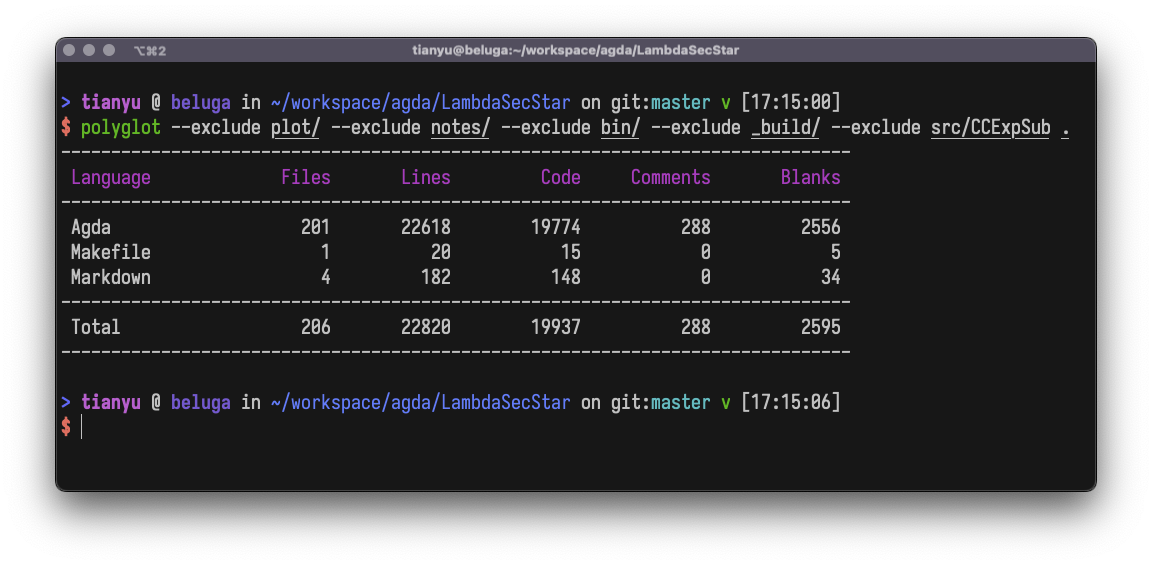
\includegraphics[width=\textwidth]{repo_stats}
\end{frame}

\begin{frame}
  \frametitle{Main Takeaways}

  \begin{enumerate}
    \item It is possible to satisfy both noninterference and the gradual guarantee
      in a gradual security-typed language,
      provided that the security level of data remains specific at runtime
      \smallskip
    \item Gradual information flow can be represented as coercions. In particular,
      NSU checking is a special projection that casts PC to the security of the memory
      location to modify
      \smallskip
    \item The key to the semantics design of of a gradual security-typed language is
      identifying injections ($\inj{\ell}$) and projections ($\proj{\ell}{p}$)
  \end{enumerate}
\end{frame}

\begin{frame}
  \centering \Large
  \redtext{Thank you} \bluetext{for your attention!}
\end{frame}

\end{document}
